%Pretend you're the investor, 
%please critically review this deck of our project.
%list the pros and cons,
%and most importantly, would you invest? 
%pretend you're the investor, give me a yes or no.


%-----

\documentclass{beamer}

\usetheme{Madrid} % You can change the theme to suit your taste

\usepackage{tikz}
\usetikzlibrary{positioning, arrows, shapes.geometric, automata, calc}
\usepackage{pgfplots}
\pgfplotsset{compat=newest}


\title{Decentralized Large AGI Model}
\author{BABEL}
\institute{P.I.V.O.T. DAO}
\date{\today}

\begin{document}

\begin{frame}
\titlepage
\end{frame}

\begin{frame}{Outline}
\tableofcontents
\end{frame}

\section{Inspiration}
\begin{frame}{Inspiration}

\begin{columns}
\column{0.6\textwidth}
Behold Babel, an artificial structure to reach for gods,  by the whole humanity across race and culture -- until gods introduced information asymmetry and distrust. 

All cryptos had to face one question: why not fiat? Eliminate criminal purposes, our answer is broader: \textbf{it must be by the whole humanity, transcending space and time}. 

While governments may fade, AGI --the unification of all human wisdom-- eternally endures.
%%%%%%%%%%%%
\column{0.4\textwidth}
\begin{center}
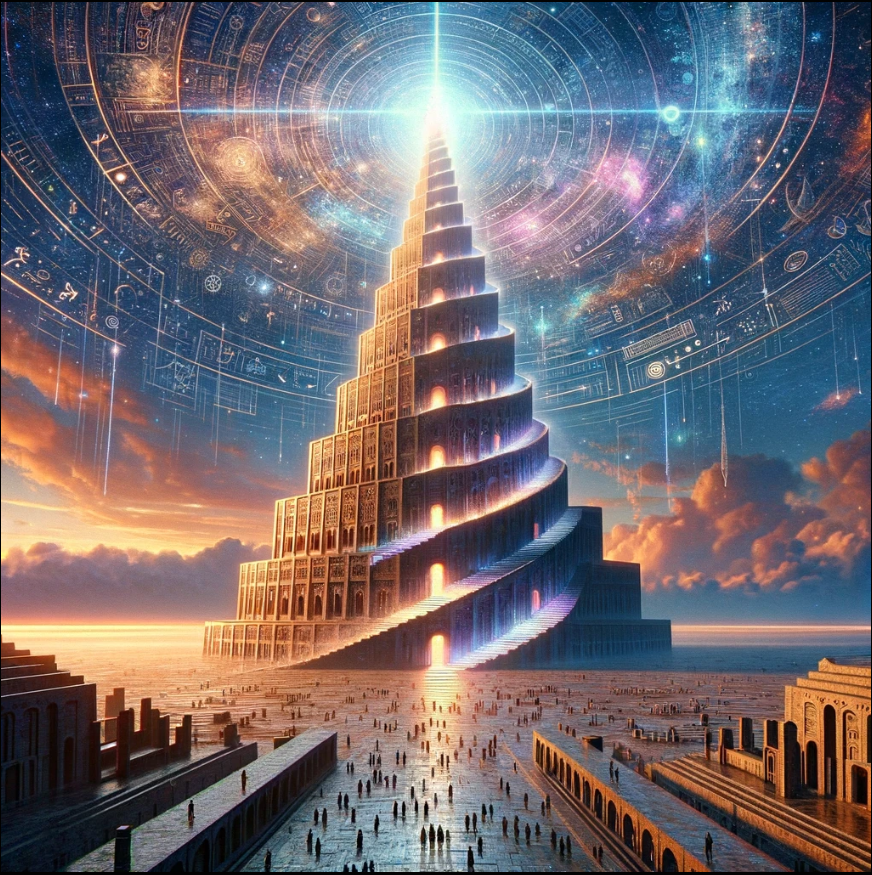
\includegraphics[width=0.9\textwidth]{images/babel.png}
\end{center}
\end{columns}

\end{frame}





% Slide 1: Purpose
\section{Purpose}
\begin{frame}{Purpose}
%\begin{itemize}
%    \item Crafting a decentralized, open-source, profitable AGI --by everyone for everyone-- combining Wikipedia-like ecosystem with a sustainable business model.
%    \item combining Wikipedia-like ecosystem with a sustainable business model.
%\end{itemize}
\begin{center}
Unify all human wisdom, by everyone for everyone, via a decentralized open-sourced \textbf{profitable} AGI 
\linebreak
\linebreak
{\scriptsize combining Wikipedia-like ecosystem with a sustainable business model}
\end{center}
\end{frame}

\section{Problems}
% Slide 2: Philosophical Problems
\begin{frame}{Philosophical Problems}
\begin{itemize}
    \item AGI (Artificial General Intelligence)--an algorithm that will outsmart humanity
    \item That's too much power for one man to have, for anyone to have.
    \item So who should own it...
    \item --everybody, I guess?
\end{itemize}
\begin{center}
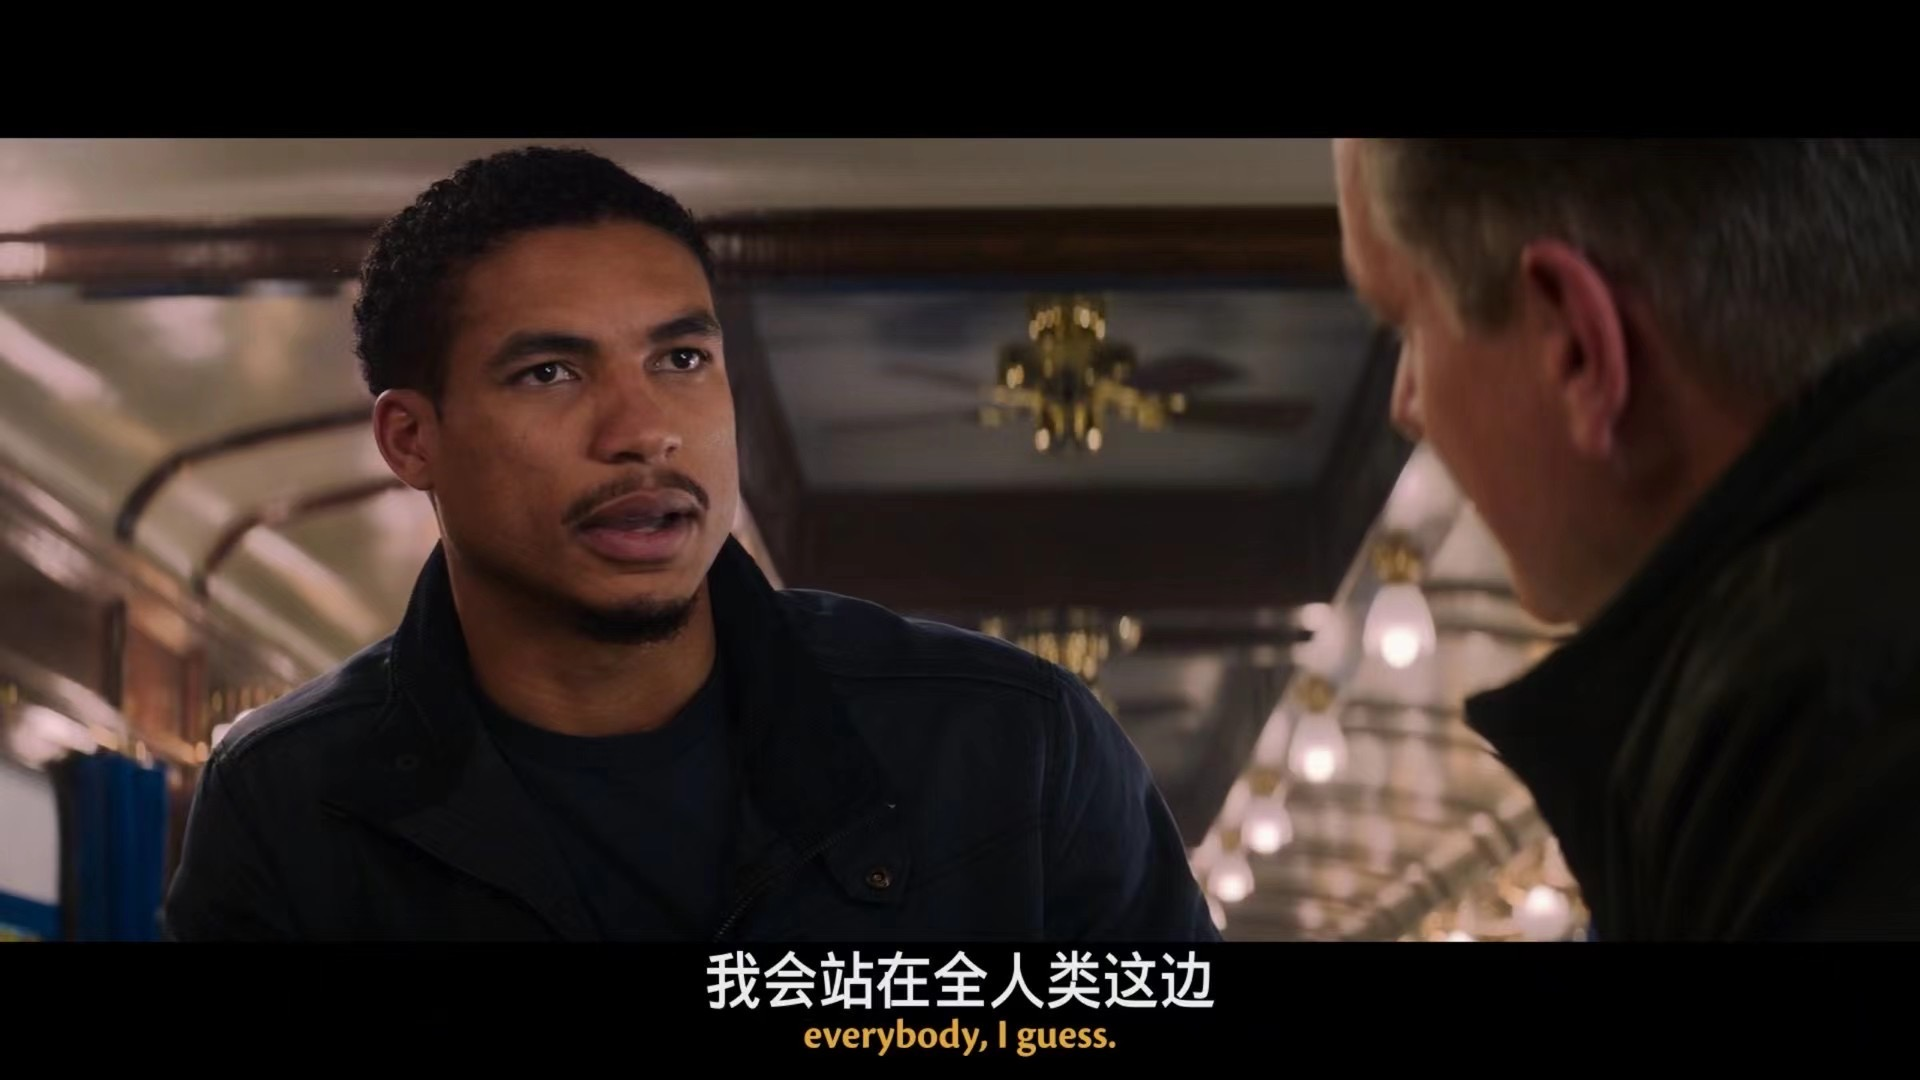
\includegraphics[width=0.5\textwidth]{images/everybody.JPG}
\end{center}
\end{frame}

% Slide 3: Specific Problems
\begin{frame}{Specific Problems}
\begin{itemize}
    \item \textbf{Centralization Risks: } A few powerful entities control AI's future, limiting diversity and innovation.
	\item \textbf{Privacy Concerns: } Inadequate protections and compensation for user data in AI development and application.
	\item \textbf{Accessibility and Economic Barriers: } High entry costs on capital prevent widespread participation in AGI's research \& development -- and applications.
	\item \textbf{Blockchain Usability: } Existing blockchain languages are hard to learn and harder to use.
	\item \textbf{Sustainability of Open-Source AGI: } Challenges in maintaining an open-source model that is both inclusive and economically viable.
\end{itemize}
\end{frame}

\section{Solution}
% Slide 4: Solution
\begin{frame}{Solution}
\begin{itemize}
    \item \textbf{Decentralized AGI Protocol: } {\footnotesize Blockchain technology decentralizes storage (data) and model training (computation)}
    \item \textbf{Personalization \& Privacy: } {\footnotesize Utilizes a foundation+personal model structure, differentiating between shared knowledge and individual, encrypted, self-owned personal models for trustless privacy.}
    \item \textbf{Fair Contribution Incentive} {\footnotesize Implements a token economy with Proof of Work of Compression (PoWoC) for quantifiable and computable contributions, reducing AGI contributors' entry barriers and encouraging wider participation.}
    \item \textbf{A+B Integration: } {\footnotesize Integrating Large Language Model (LLM) \textbf{A}GI with \textbf{B}lockchain naturally solves usability issues, making blockchain applications more accessible and applicable, fostering a sustainable, profitable, and universally fair open-source ecosystem.}
    \item \textbf{Sustainable Tokenomics: } {\footnotesize Users (demand) transfer tokens to the blockchain for A+B integration; the blockchain transfers tokens to contributors (supply) for every incremental improvement of AGI.}
\end{itemize}
\end{frame}





\section{Why Now}

% Slide: AI Trends
\begin{frame}{Why Now: AI Trends}
\begin{itemize}
    \item \textbf{Deep Blue Victory (Special-Purpose AI) \textbar 1997 \textbar} Demonstrated AI's potential in strategic games by defeating the world chess champion.
    \item \textbf{ImageNet Challenge (Special-Purpose AI) \textbar 2012 \textbar} Marked a significant milestone in computer vision, signaling the deep learning revolution.
    \item \textbf{GPT-3 Release (General-Purpose AI) \textbar 2020 \textbar} Showcased unprecedented natural language understanding and generation capabilities.
    \item \textbf{GPT-4 Release (General-Purpose AI) \textbar 2023 \textbar} Advanced the field of general-purpose AI with more sophisticated language and reasoning abilities.
\end{itemize}
\end{frame}

% Slide: Web3 Trends
\begin{frame}{Why Now: Web3 Trends}
\begin{itemize}
    \item \textbf{Bitcoin Creation \textbar 2009 \textbar} Introduced blockchain technology, launching the first decentralized digital currency.
    \item \textbf{Ethereum Launch \textbar 2015 \textbar} Brought smart contracts into play, laying the groundwork for decentralized applications.
    \item \textbf{DeFi Boom \textbar 2020 \textbar} Highlighted blockchain's potential beyond cryptocurrencies with the rapid growth in decentralized finance.
    \item \textbf{Rollups Introduction \textbar 2019-2021 \textbar} Addressed blockchain scalability, enabling faster and cheaper transactions.
\end{itemize}
\end{frame}

% Slide: Ongoing Research
\begin{frame}{Why Now: Ongoing Research}
\begin{itemize}
    \item \textbf{Layer-2 Scaling \textbar Ongoing \textbar} {\footnotesize Enhancements in scalability solutions like state channels and sidechains.}
    \item \textbf{Ethical AI Frameworks \textbar Ongoing \textbar} {\footnotesize Development of guidelines to ensure AI is developed ethically and aligned with human values.}
    \item \textbf{AGI-Rollups Concept \textbar Proposed \textbar} {\footnotesize AGI-Rollups introduce a novel approach by leveraging rollup technology for off-chain AGI computations, targeting the critical challenges of scalability and cost. This innovative integration combines the decentralized, secure infrastructure of blockchain with the expansive capabilities of AGI. It aims to revolutionize how AGI is deployed, envisioning a future where intelligent, decentralized systems are not only powered by blockchain's inherent trustlessness and resilience but are also made widely accessible and operationally efficient. }
    \item \textbf{Metaverse \textbar Emerging \textbar} {\footnotesize The  intersection of blockchain and AI paves the metaverse, a virtual shared space where users interact with a AI-generated content and other users. }
\end{itemize}
\end{frame}



\section{Market Size}
\begin{frame}{Market Size}
\begin{center}
    \Huge \$7 TRILLION \\
    \Large -- SAM ALTMAN
\end{center}
\end{frame}






\section{Competition}

\begin{frame}{Competition}
\begin{center}
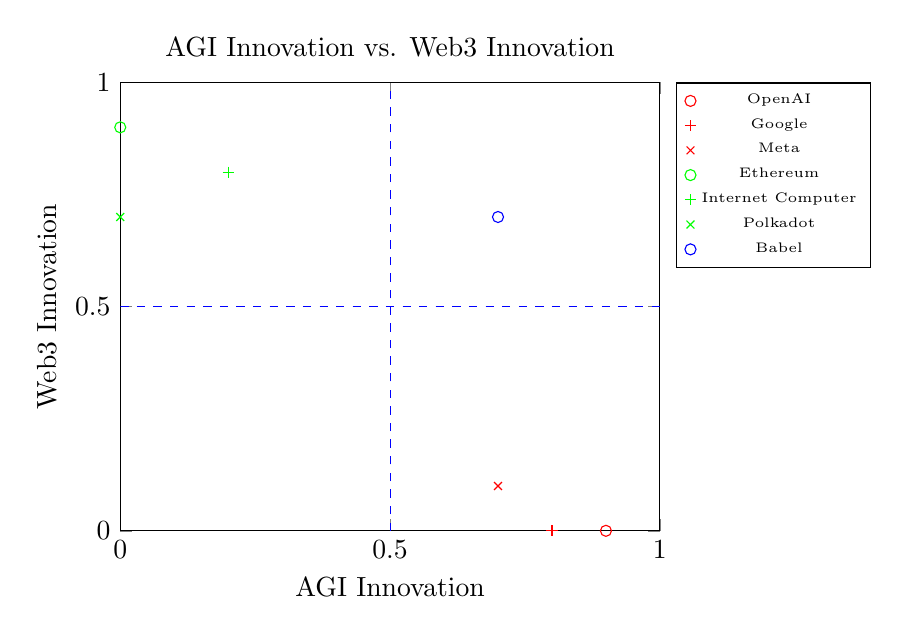
\begin{tikzpicture}
\begin{axis}[
    title={AGI Innovation vs. Web3 Innovation},
    xlabel={AGI Innovation},
    ylabel={Web3 Innovation},
    xmin=0, xmax=1,
    ymin=0, ymax=1,
    xtick={0,0.5,1},
    ytick={0,0.5,1},
    ymajorgrids=true,
    xmajorgrids=true,
    grid style=dashed,
    scatter/classes={
        a={mark=o,draw=red},
        g={mark=+,draw=red},
        m={mark=x,draw=red},
        e={mark=o,draw=green},
        i={mark=+,draw=green},
        p={mark=x,draw=green},
        b={mark=o,draw=blue}
    },
    legend style={font=\tiny},
    legend entries={OpenAI, Google, Meta, Ethereum,  Internet Computer, Polkadot, Babel},
    legend pos=outer north east,
]

% Quadrants
\draw [blue, dashed] (axis cs: 0.5,0) -- (axis cs: 0.5,1);
\draw [blue, dashed] (axis cs: 0,0.5) -- (axis cs: 1,0.5);

% Points
\addplot[scatter,only marks,scatter src=explicit symbolic]
    coordinates {
    (0.9,0) [a] % OpenAI
    (0.8,0) [g] % g
    (0.7,0.1) [m] % m
    (0,0.9) [e] % Ethereum
    (0.2,0.8) [i] % ipc
    (0,0.7) [p] % Polkadot
    (0.7,0.7) [b] % babel
};

\end{axis}
\end{tikzpicture}
\end{center}
\end{frame}





























\section{Product}


\begin{frame}{Product Components}
    \begin{itemize}
        \item \textbf{Governance DAO:} Community-driven decision-making on ecosystem proposals and policies.
        \item \textbf{Training Dataset:} Diverse datasets that grows to contain all world's data.
        \item \textbf{Compressor:} Performs Proof of Work of Compression on training dataset to optimize AGI quality and efficiency.
        \item \textbf{Compression Validator:} Ensures compressors' integrity and effectiveness of compression, and rewards tokens according to PoWoC consensus. 
        \item \textbf{AGI Rollups:} Layer-2 solution for scalable, cost-effective AGI computations on blockchain.
        \item \textbf{Babel Layer1 Chain and Miners:} Secure, decentralized, and interoperable blockchain infrastructure.
        \item \textbf{User Interface and Experience Layer:} Simplifies access to AGI applications, enhancing usability for all.
    \end{itemize}
\end{frame}






\begin{frame}{Product: PoWoC Overview}
    \begin{center}
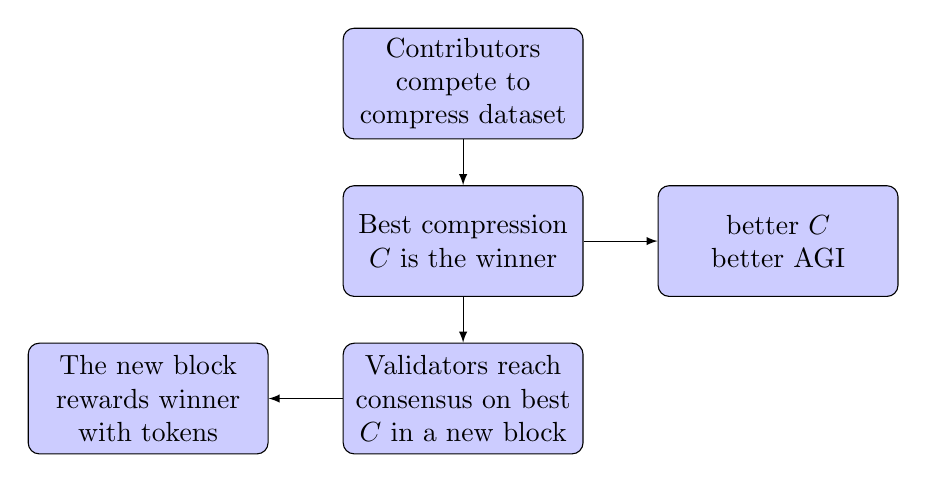
\begin{tikzpicture}[
    node distance=2cm,
    auto,
    block/.style={rectangle, draw, fill=blue!20, text width=8em, text centered, rounded corners, minimum height=4em},
    line/.style={draw, -latex}
]

% Nodes
\node[block] (miner) {Contributors compete to compress dataset};
\node[block, below of=miner] (winner) {Best compression $C$ is the winner};
\node[block, below of=winner] (validators) {Validators reach consensus on best $C$ in a new block};
\node[block, right of=winner, xshift=2cm] (agi) {better $C $\\  better AGI};
\node[block, left of=validators, xshift=-2cm] (reward) {The new block rewards winner with tokens};

% Paths
\path[line] (miner) -- (winner);
\path[line] (winner) -- (validators);
\path[line] (winner) -- (agi);
\path[line] (validators) -- (reward);

\end{tikzpicture}
    \end{center}
\end{frame}





\begin{frame}{Product Features}
    \begin{itemize}
        \item \textbf{Decentralized Architecture}: Blockchain ensures security, transparency, and tamper-proof ecosystem interactions.
        \item \textbf{AGI-Embedded Intelligent Contract}: Integrates AGI with smart contracts for adaptive, privacy-enhanced, intelligent decision-making.
        \item \textbf{Personalized \& Private AGI Agent}: Offers user-specific AGI agents for customized interactions and advanced privacy.
        \item \textbf{Token Economy \& Dynamic Participation}: A novel token model rewards participation, enabling a vibrant community where users are both demanders and suppliers.
        \item \textbf{Scalable and Efficient}: Utilizes AGI-Rollups to address scalability and transaction cost challenges, ensuring platform efficiency.
        \item \textbf{Open Development Platform}: Provides tools for creating AGI-driven applications, fostering innovation and ecosystem growth.
        \item \textbf{Ethical and Transparent AI Use}: Committed to ethical AI practices, ensuring transparency and equitable benefits for all.
    \end{itemize}
\end{frame}









\begin{frame}{Product Roadmap}
    \footnotesize % Adjust the font size to fit the content on the slide
    \begin{itemize}
        \item \textbf{Q1-Q2 2024:}
        \begin{itemize}
            \item Launch of AGI-Rollups Beta and PoWoC Beta for scalable blockchain operations.
            \item Initial Token Distribution Event to early adopters.
        \end{itemize}
        
        \item \textbf{Q3-Q4 2024:}
        \begin{itemize}
            \item Personalized AGI Agents Beta
            \item Expansion of Developer Tools with new SDKs and APIs.
        \end{itemize}
        
        \item \textbf{Q1-Q2 2025:}
        \begin{itemize}
            \item Integration with Major Blockchain Platforms for increased interoperability.
            \item Launch of Decentralized Marketplace for AGI-driven services.
        \end{itemize}
        
        \item \textbf{Q3-Q4 2025:}
        \begin{itemize}
            \item Implementation of Ethical AI Governance Framework.
            \item Hosting of Global AGI Conference to foster community collaboration.
        \end{itemize}
        
        \item \textbf{Beyond 2025:}
        \begin{itemize}
            \item Continuous Improvement and Expansion of AGI capabilities and platform features.
        \end{itemize}
    \end{itemize}
\end{frame}












\section{Business Model}
\begin{frame}[t]{Business Model: Ecosystem as a Service}
    \textit{An ecosystem of an AGI-embedded blockchain for more casual use}
    
    %\vspace{10pt} % Adjust space as needed

    \begin{center}
    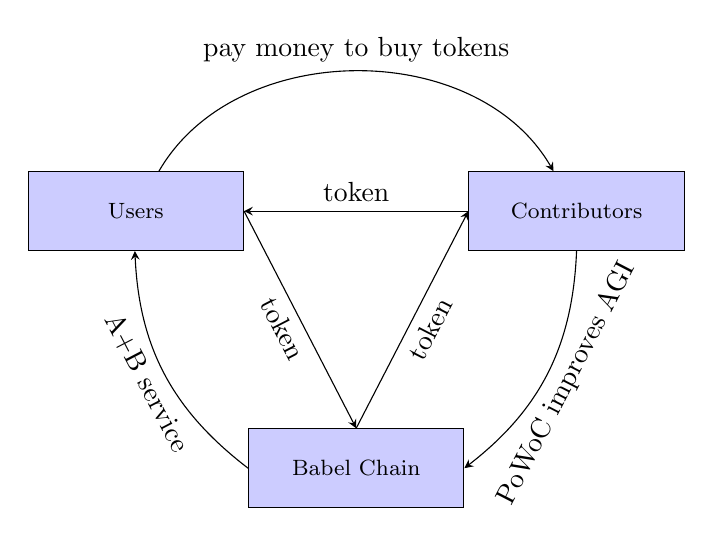
\begin{tikzpicture}[>=stealth, node distance=0.25cm and 0.5cm, 
    block/.style={rectangle, draw, text width=2.5cm, align=center, minimum height=1cm, fill=blue!20, font=\footnotesize}]
    
    % Nodes
    \node[block] (babel) {Babel Chain};
    \node[block, above left=of babel, yshift=2cm, xshift=0.45cm] (users) {Users};
    \node[block, above right=of babel, yshift=2cm, xshift=-0.45cm] (contributors) {Contributors};
    
    % Paths
    \draw[->] (users.east) to[bend left=0] node[below, sloped] { token} (babel.north);
    \draw[->] (babel.north) to[bend left=0] node[below, sloped] { token} (contributors.west);
    \draw[->] (contributors.west) to[bend left=0] node[above, sloped] { token} (users.east);
    
    
    \draw[->] (contributors.south) to[bend left=25] node[below, sloped] {PoWoC improves AGI} (babel.east);


    \draw[->] (users) to[bend left=60] node[above, sloped] {pay money to buy tokens} (contributors);

    % Additional Information
    \draw[->] (babel.west) to[bend left=25] node[below, sloped] { A+B service} (users);
    
    \end{tikzpicture}
    \end{center}
\end{frame}
































\section{Conclusion}
\begin{frame}{Key Take-away}
Satoshi found a metric to compute degrees of faithfulness: \textbf{PoW}

Vitalik found a metric to compute degrees of loyalty: \textbf{PoS}

We found a metric to compute degrees of intelligence: \textbf{PoWoC}
\end{frame}



\section{FAQ}
\begin{frame}{FAQ}
\textbf{Q: Can someone with no hardware participate in PoWoC?} \\
A: Yes, tweaking the prompts might also cause surprising effects on the compression ratio, making participation feasible even without specialized hardware. In fact, there are various means to earn tokens in the ecosystem, all but the first one is strongly related to PoWoC:
\begin{itemize}
\item contribute data
\item contribute computing power \#PoWoC \#hardware
\item revise prompts \#PoWoC
\end{itemize}
\end{frame}


\end{document}



